\documentclass[twoside]{article}
\usepackage[a4paper]{geometry}
\geometry{verbose,tmargin=2.5cm,bmargin=2cm,lmargin=2cm,rmargin=2cm}
\usepackage{fancyhdr}
\pagestyle{fancy}

% nastavení pisma a~češtiny
\usepackage{lmodern}
\usepackage[T1]{fontenc}
\usepackage[utf8]{inputenc}
\usepackage[czech]{babel}

% odkazy
\usepackage{url}

\usepackage{float}
% vícesloupcové tabulky
\usepackage{multirow}
\usepackage{listings}
\usepackage{xcolor}
\usepackage{amssymb}
\usepackage{gensymb}
\usepackage{bbold}
\usepackage{amsmath}
\usepackage{siunitx}
\usepackage{mathtools}
\usepackage{commath}

% vnořené popisky obrázků
\usepackage{subcaption}

% automatická konverze EPS 
\usepackage{graphicx} 
\usepackage{epstopdf}
\epstopdfsetup{update}

\graphicspath{{./images}}

% odkazy a~záložky
\usepackage[unicode=true, bookmarks=true,bookmarksnumbered=true,
bookmarksopen=false, breaklinks=false,pdfborder={0 0 0},
pdfpagemode=UseNone,backref=false,colorlinks=true] {hyperref}


% Poznámky při překladu
\usepackage{xkeyval}	% Inline todonotes
\usepackage[textsize = footnotesize]{todonotes}
\presetkeys{todonotes}{inline}{}

%https://tex.stackexchange.com/questions/2783/bold-calligraphic-typeface
\DeclareMathAlphabet\mathbfcal{OMS}{cmsy}{b}{n}

% enumerate zacina s pismenem
\renewcommand{\theenumi}{\alph{enumi}}
\newcommand{\Cx}{C_{\rm x}}
\newcommand{\Rx}{R_{\rm x}}

% smaz aktualni page layout
\fancyhf{}
% zahlavi
\usepackage{titling}
\fancyhf[HC]{\thetitle}
\fancyhf[HLE,HRO]{\theauthor}
\fancyhf[HRE,HLO]{27. května 2022}
 %zapati
\fancyhf[FLE,FRO]{\thepage}

% údaje o autorovi
\title{OTE Semestrální úloha -- Kapacitní snímač výšky hladiny}
\author{Vojtěch Michal}
\date{27. května 2022}

%customize code listing
\definecolor{codegreen}{rgb}{0,0.6,0}
\definecolor{codegray}{rgb}{0.5,0.5,0.5}
\definecolor{codepurple}{rgb}{0.58,0,0.82}
\definecolor{backcolour}{rgb}{0.95,0.95,0.92}

\lstdefinestyle{mystyle}{
    backgroundcolor=\color{backcolour},   
    commentstyle=\color{codegreen},
    keywordstyle=\color{magenta},
    numberstyle=\tiny\color{codegray},
    stringstyle=\color{codepurple},
    basicstyle=\ttfamily\footnotesize,
    breakatwhitespace=false,         
    breaklines=true,                 
    captionpos=b,                    
    keepspaces=true,                 
    numbers=left,                    
    numbersep=5pt,                  
    showspaces=false,                
    showstringspaces=false,
    showtabs=false,                  
    tabsize=2
}

\lstset{style=mystyle}

\begin{document}

\maketitle

\section{Přenos kapacitního snímače}

Pro odvození přenosu kapacitního snímače z
budicího napětí $U_1$ (uzel \textit{buzeni} ve schématu \ref{schema}) na výstupní napětí $U_2$ (uzel 15  ve schématu \ref{schema})
je použit virtuální zkrat mezi vstupy operačního zesilovače U3A
s imedančním děličem ve zpětné vazbě.
Nechť $Z_A$ označuje impedanci obecného prvku $A$, poté se dá virtuální zkrat vstupů popsat rovnicí
\begin{equation}
    U_1 = U_2 \cdot \frac{Z_{\Cx} || Z_{\Rx}}{(Z_{\Cx} || Z_{\Rx}) + Z_{C_1}}.
\end{equation}
Odtud je přenos ze vstupu na výstup roven
\begin{equation}
    \begin{aligned}
        \frac{U_2}{U_1} &= \frac{(Z_{\Cx} || Z_{\Rx}) + Z_{C_1}}{Z_{\Cx} || Z_{\Rx}} 
        &= \frac{\frac{\frac{\Rx}{j\omega \Cx}}{\Rx + \frac{1}{j\omega \Cx}} + \frac{1}{j\omega C_1}}{ \frac{\frac{\Rx}{j\omega \Cx}}{\Rx + \frac{1}{j\omega \Cx}}   } \\
        &= \frac{\frac{\Rx}{\Rx j\omega \Cx + 1} + \frac{1}{j\omega C_1}}{ \frac{\Rx}{\Rx j\omega \Cx + 1}   }
        &= \frac{\frac{\Rx j \omega \Cx + 1 + \Rx j \omega C_1}{j\omega C_1(1 + \Rx j\omega \Cx)}}{\frac{\Rx}{j\omega \Cx \Rx  + 1}} \\
        &= \frac{1 + \Rx j \omega (\Cx +C_1)}{j\omega \Rx C_1} 
        &= \frac{1}{j\omega \Rx C_1} + \frac{\Cx +C_1}{C_1} \\
        &= \frac{\Cx + C_1}{C_1} - j \frac{1}{\omega \Rx C_1}.
    \end{aligned}
\end{equation}

Pro měření neznámé kapacity $\Cx$ je tak postačující synchronním detektorem
sledovat reálnou složku výstupního signálu (spínač bude řízen ve fázi s budicím signálem),
jež bude afinní funkcí neznámé kapacity
\begin{equation}
    U_{\rm out} = \left(1 + \frac{\Cx}{C_1}\right) U_{\rm in}.
    \label{eq:zesileni}
\end{equation}
Velikost ztrátového odporu $\Rx$ nemá ideálně na měřenou reálnou složku žádný vliv.

\clearpage
\section{Návrh obvodu}


Pro praktickou realizaci byl použit obvod Wienova oscilátoru napájeného z $\pm \SI{5}{\volt}$,
kterému je ve zpětné vazbě nastaven trimmer R1 na 38 \% rozsahu \SI{50}{\kilo\ohm}
tak, aby budicí signál měl amplitudu \SI{1}{\volt}.
Pro rozkmitání obvodu je potřeba na okamžik snížit nastavení R1 na 37 \% rozsahu.
Měřicí obvod je postaven ze
čtyřnásobného operačního zesilovače TL084CD (součástka U3A) 
a jako spínač v synchronním detektoru
je použit NPN tranzistor BC548BP (součástka Q1).


V měřicí části obvodu, viditelné na obrázku \ref{schema}, je buzení 
vedeno na neinvertující vstup U3A, v jehož zpětné vazbě je 
zapojena měřená impedance $\Rx,~\Cx$. Byla zvolena kapacita $C_1 = \SI{300}{\pico\farad}$,
aby bylo zesílení měřicího obvodu dle rovnice \eqref{eq:zesileni} omezeno na rozsah 1 až 2
a nedocházelo tak k saturaci operačního zesilovače, který dle produktového listu není
rail-to-rail.

\begin{figure}[h]
    \centering
    \includegraphics[width=\textwidth]{schema.png}
    \caption{Simulační schéma}
    \label{schema}
\end{figure}

Kanál U3B slouží jako zesilovač s přepínatelným zesílením $\pm 1$, jehož spínající
tranzistor je řízen kanálem U3D použitým v roli komparátoru budicího signálu s nulou.
Poslední kanál v pouzdře TL084 je použit jako sčítací zesílovač, který odstraňuje
experimentálně naměřenou stejnosměrnou složku \SI{1070}{\milli\volt} z
výstupu synchronního detektoru a zajišťuje, že výstup 
celého obvodu (uzel 15) je v rozsahu 0 až 1 V dle požadavků zadání.
Pro realizaci obvodu byla zvolena řada odporů E24, proto dělič R11, R12
s výstupím napětím \SI{1070}{\milli\volt} sestává z odporů \SI{1100}{\ohm} a \SI{300}{\ohm}
a ve zpětné vazbě U3C je odpor \SI{192}{\kilo\ohm}, jenž lze vytvořit seriovým zapojením
odporů \SI{180}{\kilo\ohm} a \SI{12}{\kilo\ohm}.


\clearpage

\section{Měření kapacity $\Cx$}

\subsection{Harmonické buzení bez rušení}
Bez připojení rušivého napětí byla změřena charakteristika uvedená v tabulce \ref{tab:mereni-c}
a na obrázku \ref{fig:mereni-c}. Směrodatná odchylka od ideální lineární
převodní charakteristiky je $\sigma = \SI{8.7}{\milli\volt}$ a rozptyl
$\sigma^2 = \SI{75.78}{\milli\volt\squared}$.

\begin{figure}[h]
    \centering
    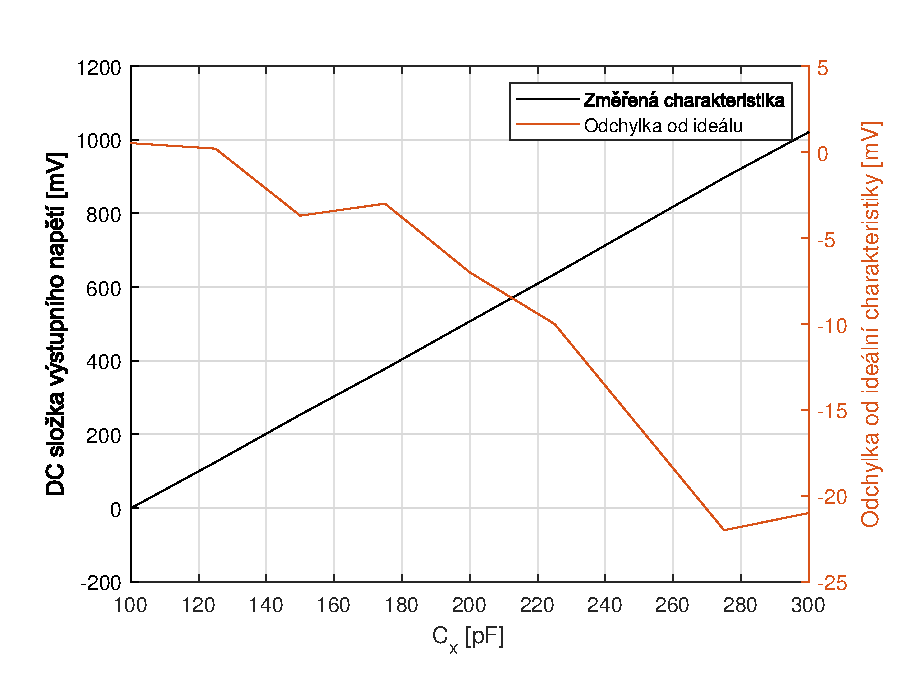
\includegraphics[width=\textwidth]{mereni-c.eps}
    \caption{Převodní charakteristika z kapacity $\Cx$ na výstup bez rušení}
    \label{fig:mereni-c}
\end{figure}

\begin{table}[h]
    \centering
    \begin{tabular}{c|c|c|c}
        kapacita $\Cx$ [pF] & Změřený výstup [mV] & Ideální výstup [mV] & Odchylka [mV] \\\hline
    100 &  -0.5  &       0 &   0.5 \\
    125 &   124  &  125 &      0.2\\
    150 &   253  &  250 &     -3.7\\
    175 &   378  &  375 &     -3 \\
    200 &   507  &  500 &     -7 \\
    225 &   635  &  625 &    -10 \\
    250 &   766  &  750 &    -16 \\
    275 &   897  &  875 &    -22 \\
    300 &   1021  &  1000 &  -21 \\        
    \end{tabular}
    \caption{Změřené body převodní charakteristiky z kapacity $\Cx$ na výstup bez rušení}
    \label{tab:mereni-c}
\end{table}

\clearpage
\subsection{Harmonické buzení s rušením}

Po připojení rušivého napětí o amplitudě \SI{100}{\milli\volt} a frekvenci \SI{50}{\hertz}
byly změřeny body charakteristiky uvedené v tabulce \ref{tab:mereni-c-noise}
a na grafu \ref{fig:mereni-c-noise}. 
Je vidět, že rušivé napětí způsobilo
přibližně lineárně rostoucí odchylku od měření provedeného bez rušení (tabulka \ref{tab:mereni-c}),
jejíž směrodatná odchylka je $\sigma = \SI{16.74}{\milli\volt}$ a rozptyl
$\sigma^2 = \SI{280.48}{\milli\volt\squared}$.
Je očekávatelné, že je na výstupu odlišné napětí, protože modulované rušení
způsobilo nepřesnost synchronní detekce. Proto se na výstup začala propisovat
i imaginární složka signálu.

\begin{figure}[h]
    \centering
    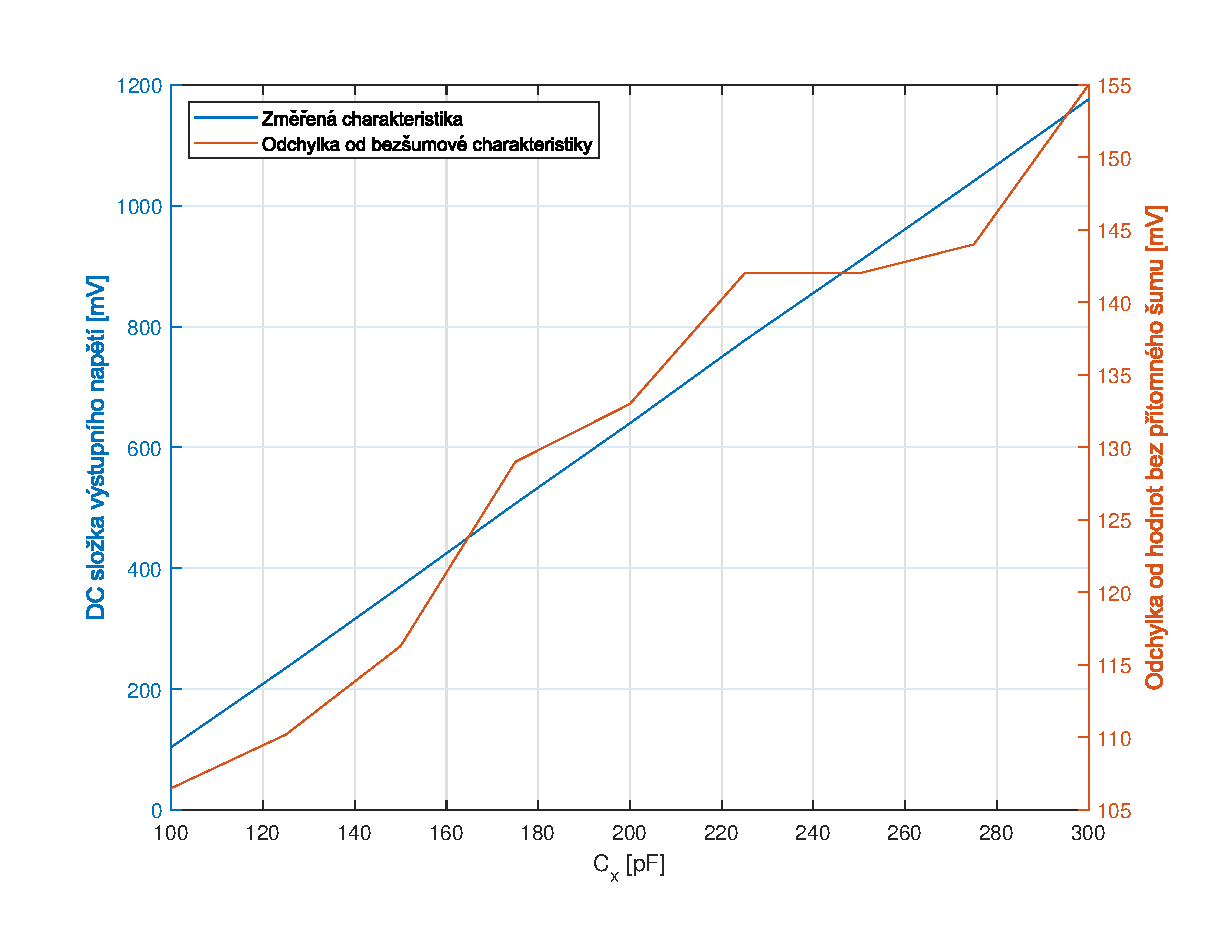
\includegraphics[width=\textwidth]{mereni-c-noise.eps}
    \caption{Převodní charakteristika z kapacity $\Cx$ na výstupní napětí s rušením}
    \label{fig:mereni-c-noise}
\end{figure}

\begin{table}[h]
    \centering
    \begin{tabular}{c|c|c|c}
        kapacita $\Cx$ [pF] & Změřený výstup [mV] & Ideální výstup [mV] & Odchylka [mV] \\\hline
      
    \end{tabular}
    \caption{Změřené body převodní charakteristiky z kapacity $\Cx$ na výstupní napětí s rušením}
    \label{tab:mereni-c-noise}
\end{table}

\subsection{Obdélníkové buzení}

Při buzení obvodu pomocí \textit{clock voltage} o frekvenci \SI{1}{kHz} a amplitudě \SI{1}{V}
se nepodařilo změřit žádné rozumné charakteristiky,
protože výstupy operačních zesilovačů rychle odcházely do saturace
bez zřejmé závislosti na velikosti neznámé kapacity $\Cx$.

\clearpage

\section{Potlačení změny $Rx$}

Výstupní napětí by dle \eqref{eq:zesileni} mělo být málo závislé
na velikosti ztrátového odporu $\Rx$. V tabulce \ref{tab:mereni-r}
a na grafu \ref{fig:mereni-r} jsou zachyceny body převodní charakteristiky obvodu.
Hodnoty v grafu jsou vztaženy k "ideálním" hodnotám naměřeným při největším nastaveném odporu
$\Rx = \SI{10}{\mega\ohm}$.

\begin{figure}[h]
    \centering
    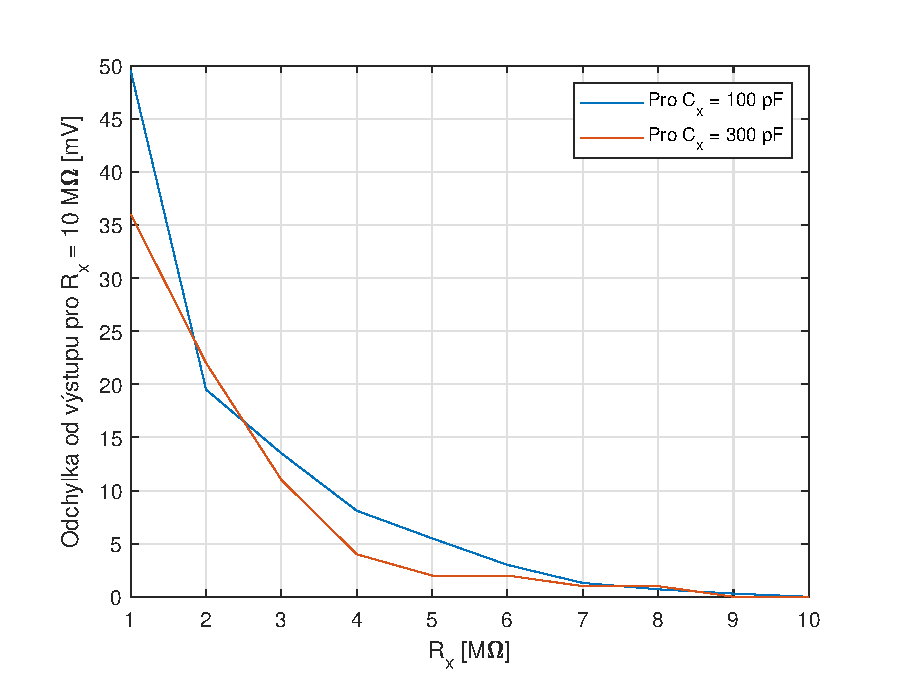
\includegraphics[width=0.8\textwidth]{mereni-r.eps}
    \caption{Převodní charakteristika z odporu $\Rx$ na výstup}
    \label{fig:mereni-r}
\end{figure}

\begin{table}[h]
    \centering
    \begin{tabular}{c|c|c|c}
        odpor $\Rx$ [M$\Omega$] & Výstup pro $\Cx = \SI{100}{\pico\farad}$ [mV] & Výstup pro $\Cx = \SI{300}{\pico\farad}$ [mV] \\\hline
        1  &  47  &  1055 \\
        2  &  17  &  1041 \\
        3  &  11  &  1030 \\
        4  &  5.6  &  1023 \\
        5  &  3.0  &  1021 \\
        6  &  0.5  &  1021 \\
        7  & -1.2  &  1020 \\
        8  & -1.8  &  1020 \\
        9  & -2.2  &  1019 \\
        10 &  -2.5 &   1019 \\
    \end{tabular}
    \caption{Změřené body převodní charakteristiky z odporu $\Rx$ na výstup}
    \label{tab:mereni-r}
\end{table}


\end{document}

